\section{Forecast computation}
In order to do a realistic study for the new Bekasi-East airport traffic, it is previously established the Soekarno-Hatta International Airport (CGK) as the reference airport for future operations prevision. According to one of the IATA main recommended methods for the elaboration of traffic previsions, data from historical series of CGK traffic has been used so as to be able to extrapolate the study horizons of the airport to be designed.

In order to do this, it is necessary to calculate the annual variation tendency of the different traffic parameters from historical data of the last years. Data mentioned is extracted from the "Directorate General of Civil Aviation" (DGCA) and "FlightRadar24" web pages.

With this information, the next step is to calculate the values of horizon scenario, which has been fixed in 15 years with respect to the airport inauguration (it is expected to be finished in 2020). The horizon scenario will be fixed then in 2035.  

Before starting the study of passenger and operation demands, some important aspects will be taken into account:

\begin{itemize}
	\item The airport to be projected will absorb nearly the 40\% of CGK’s current traffic, which corresponds to the percentage of delayed flights due to congestion.
	\item The growth tendencies, concretely the Compound Annual Growth Rate (CAGR), has been calculated using the data corresponding to the five more recent years. The expression used to calculate the values is the following one:
	\begin{equation}
	CAGR=\left(\frac{V_{fin}}{V_{ini}}\right)^{\frac{1}{t_{fin}-t_{ini}}}-1
	\end{equation}
	\item The prediction of passengers and operations have been calculated using three possible scenario.
	\begin{itemize}
		\item Neutral scenario: The growth is constant along time. This neutral scenario has been used to estimate the number of passengers and operations in 2035.
		\item Optimistic scenario: The growth is constant along time but in 2025 is multiplied by a factor of 1,5 due to, for example, a boom of tourism in the city.
		\item Pessimistic scenario: The growth is constant along time but in 2025 is divided by a factor of 2 due to, for example, a period of time with adverse atmospheric phenomena.
	\end{itemize}
\end{itemize}

In addition, both the airlines as well as the percentage of operations absorbed from CGK are detailed in the following table:

	\begin{table}[ht!]
	\label{table:AirlinesAbsorbed}
	\centering
	\begin{tabular}{|c|c|}
		\hline
		\textbf{AIRLINES} & \textbf{\% OPERATIONS}\\
		\hline
		\textbf{Garuda} & 31.62\\
		\hline
		\textbf{Citilink} & 7.11\\
		\hline
		\textbf{Emirates} & 0.35\\
		\hline
		\textbf{Etihad} & 0.44\\
		\hline
		\textbf{Qatar} & 0.53\\
		\hline
		\textbf{Total} & 40.05\\
		\hline
	\end{tabular}
	\caption{Airlines absorbed and operation percentages from CGK.}
	\end{table}

	\subsection{Passenger prediction}
In this section it will be calculated the number of annual passenger both domestic and international in the horizon scenario in 2035.
 
Taking into account the historical passenger data collected from CGK airport, one can obtain:

\begin{table}[ht!]
	\label{table:PAXCGK}
	\centering
\begin{tabular}{|c|c|c|c|}
	\hline 
	\textbf{Year} & \textbf{Domestic PAX} & \textbf{International PAX} & \textbf{Total PAX}\tabularnewline
	\hline 
	\textbf{2011} & 35.412.018  & 10.589.310  & 46.001.328 \tabularnewline
	\hline 
	\textbf{2012} & 39.499.760  & 11.674.136  & 51.173.896 \tabularnewline
	\hline 
	\textbf{2013} & 41.318.616  & 12.743.330  & 54.061.946 \tabularnewline
	\hline 
	\textbf{2014} & 40.531.384  & 12.489.680  & 53.021.064 \tabularnewline
	\hline 
	\textbf{2015} & 38.262.800  & 12.696.766  & 50.959.566 \tabularnewline
	\hline 
\end{tabular}
	\caption{Volume of passengers of the last 5 years in CGK Airport.}
\end{table}

The CAGR's calculated from  data in the table above:
 \begin{itemize}
 	\item CAGR for Neutral Scenario
 	
\begin{table}[ht!]
	\label{table:CAGRNeutralPAX}
	\centering
	\begin{tabular}{|c|c|c|c|}
		\hline 
		\textbf{Type} & \textbf{Initial Value} & \textbf{Final Value} & \textbf{PAX CAGR}\tabularnewline
		\hline 
		Domestic & 35.412.018  & 38.262.800  & 1,95\% \tabularnewline
		\hline 
		International & 10.589.310  & 12.696.766  & 4,64\% \tabularnewline
		\hline 
	\end{tabular}
	\caption{Neutral scenario passenger CAGR.}
\end{table}
 	
 	\item CAGR for Optimistic and Pessimistic Scenario (applied from 2025)
 	
\begin{table}[ht!]
	\label{table:CAGROPTPESPAX}
	\centering
	\begin{tabular}{|c|c|c|}
		\hline 
		\textbf{Type} & \textbf{Optimistic PAX CAGR} & \textbf{Pessimistic PAX CAGR}\tabularnewline
		\hline 
		Domestic & 2,93\%  & 0,98\% \tabularnewline
		\hline 
		International & 6,96\%  & 2,32\% \tabularnewline
		\hline 
	\end{tabular}
	\caption{Optimistic and pessimistic scenario passenger CAGR.}
\end{table}
 \end{itemize}
	
Using the growth taxes computed previously, it is obtained the following results in horizon scenario.

\begin{figure}[H]
	\centering
	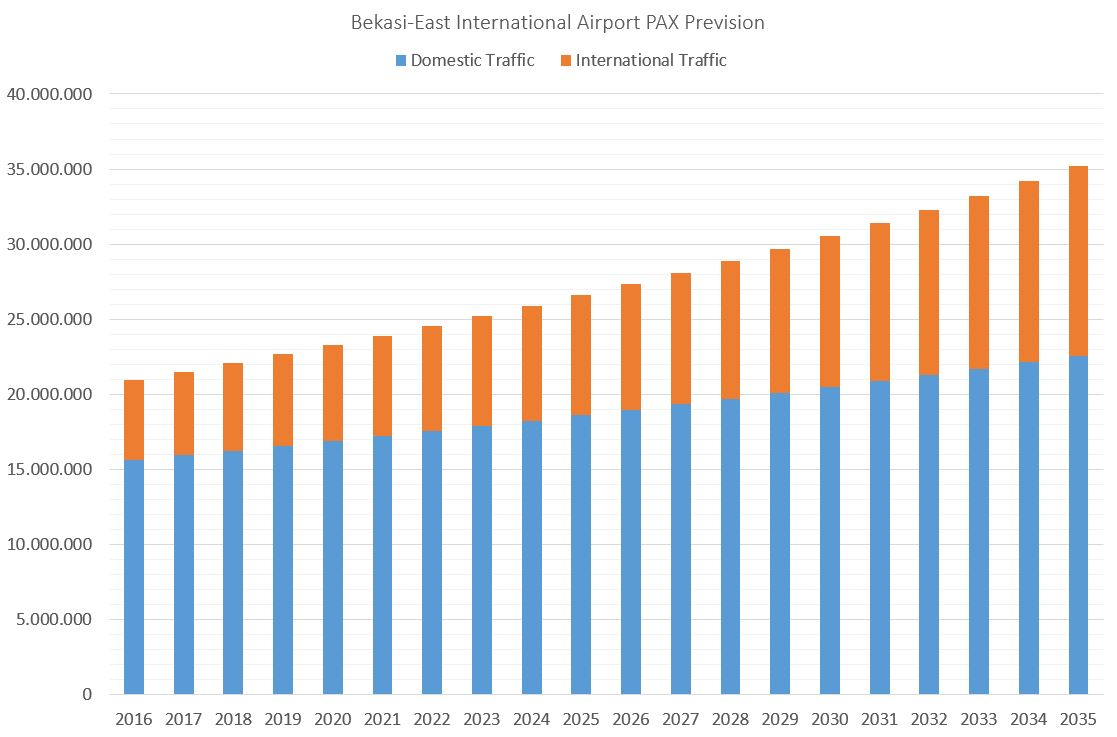
\includegraphics[clip, trim=0cm 0cm 0cm 0cm, width=1\textwidth]{./images/PROGNOSIS/TrafficForecast/BE_PAX_Prev}
	\caption{Bekasi-East Jakarta Airport passenger prevision.}
	\label{BE_PAX_Prev}
\end{figure}

\begin{figure}[H]
	\centering
	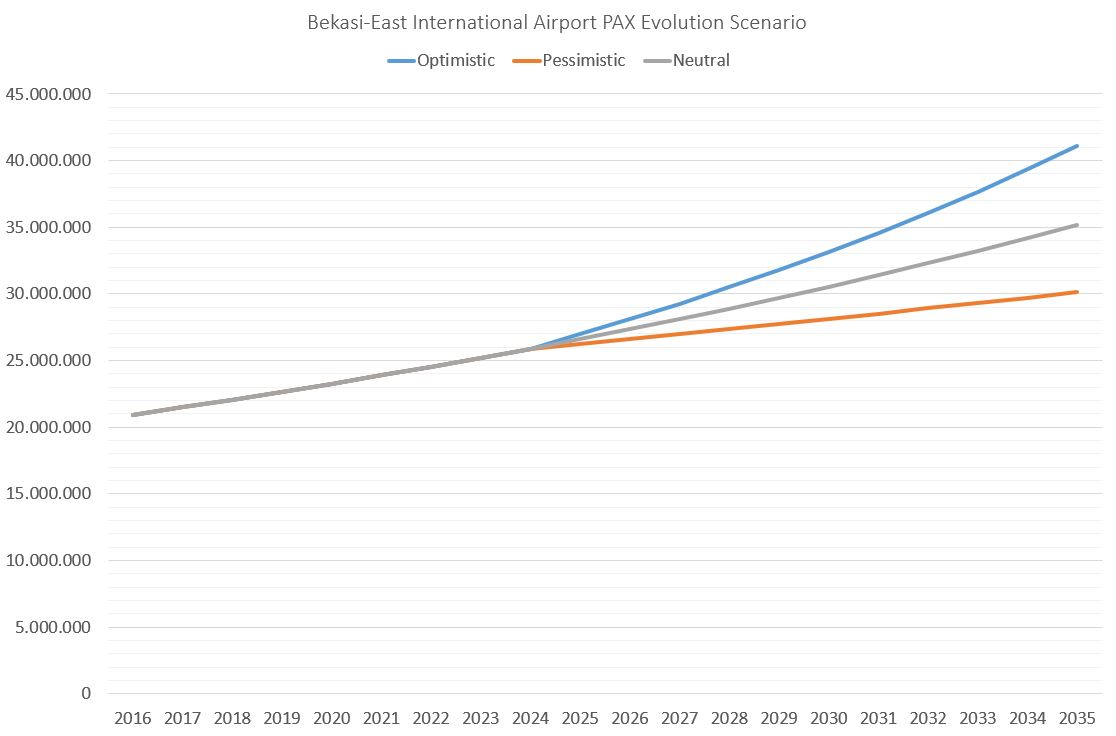
\includegraphics[clip, trim=0cm 0cm 0cm 0cm, width=1\textwidth]{./images/PROGNOSIS/TrafficForecast/BE_PAX_Prev_NEUOPTPES}
	\caption{Bekasi-East Jakarta Airport passenger prevision for neutral, optimistic and pessimistic scenario.}
	\label{BE_PAX_Prev_NEUOPTPES}
\end{figure}

	\subsection{Operations prediction}
In this section it will be calculated the number of annual operations both domestic and international in the horizon scenario in 2035.
	
Taking into account the historical operations data collected from CGK airport, one can obtain:

\begin{table}[ht!]
	\label{table:OPSCGK}
	\centering
\begin{tabular}{|c|c|c|c|}
	\hline 
	\textbf{Year} & \textbf{Domestic OPS} & \textbf{International OPS} & \textbf{Total OPS}\tabularnewline
	\hline  
	\textbf{2011} & 279.668  & 68.241  & 347.909 \tabularnewline
	\hline 
	\textbf{2012} & 327.416  & 79.288  & 406.704 \tabularnewline
	\hline 
	\textbf{2013} & 329.568  & 82.924  & 412.492 \tabularnewline
	\hline 
	\textbf{2014} & 331.120  & 115.184  & 446.304 \tabularnewline
	\hline 
	\textbf{2015} & 301.696  & 84.919  & 386.615 \tabularnewline
	\hline 
\end{tabular}
	\caption{Volume of operations of the last 5 years in CGK Airport.}
\end{table}
	
The CAGR's calculated from  data in the table above:
	\begin{itemize}
		\item CAGR for Neutral Scenario
		
\begin{table}[ht!]
	\label{table:CAGRNeutralOPS}
	\centering
\begin{tabular}{|c|c|c|c|}
	\hline 
	\textbf{Type} & \textbf{Initial Value} & \textbf{Final Value} & \textbf{OPS CAGR}\tabularnewline
	\hline 
	Domestic & 279.668  & 301.696  & 1,91\% \tabularnewline
	\hline 
	International & 68.241  & 84.919  & 5,62\% \tabularnewline
	\hline 
\end{tabular}
	\caption{Neutral scenario operations CAGR.}
\end{table}
		
		\item CAGR for Optimistic and Pessimistic Scenario (applied from 2025)
		
\begin{table}[ht!]
			\label{table:CAGROPTPESOPS}
			\centering
	\begin{tabular}{|c|c|c|}
		\hline 
		\textbf{Type} & \textbf{Optimistic OPS CAGR} & \textbf{Pessimistic OPS CAGR}\tabularnewline
		\hline  
		Domestic & 2,87\%  & 0,96\% \tabularnewline
		\hline 
		International & 8,43\%  & 2,81\% \tabularnewline
		\hline 
\end{tabular}
			\caption{Optimistic and pessimistic scenario operations CAGR.}
		\end{table}
		
	\end{itemize}
	
Using the growth taxes computed previously, it is obtained the following results in horizon scenario.
	
\begin{figure}[H]
	\centering
	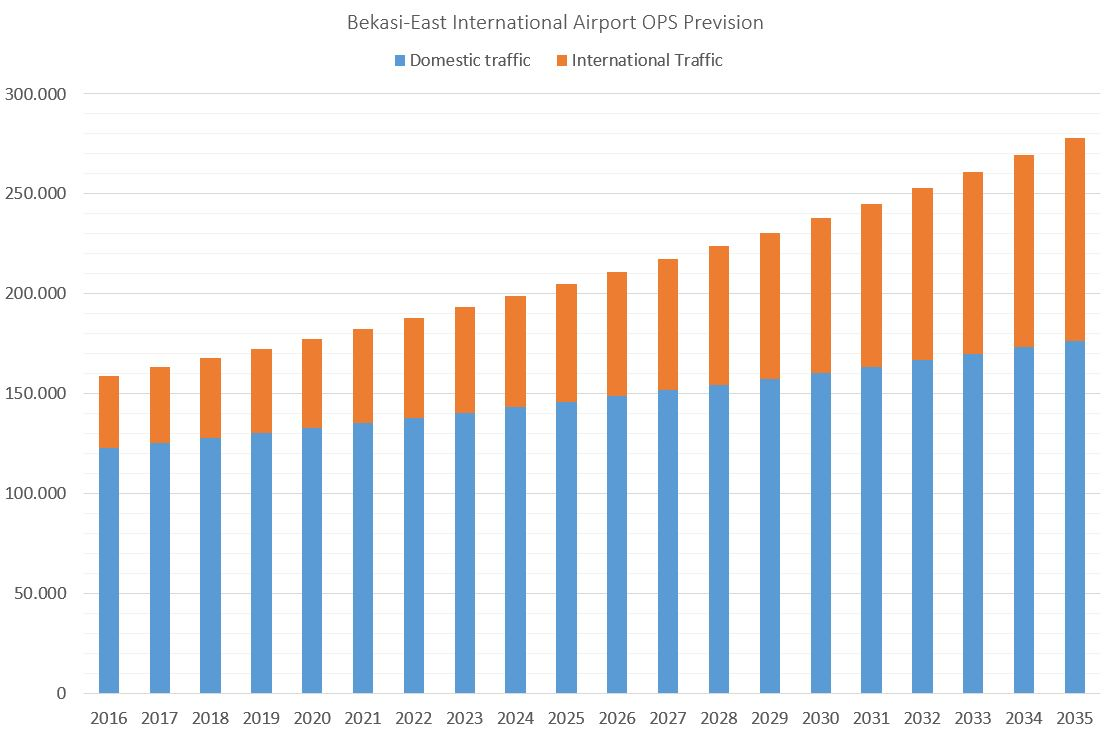
\includegraphics[clip, trim=0cm 0cm 0cm 0cm, width=1\textwidth]{./images/PROGNOSIS/TrafficForecast/BE_OPS_Prev}
	\caption{Bekasi-East Jakarta Airport operations prevision.}
	\label{BE_OPS_Prev}
\end{figure}

\begin{figure}[H]
	\centering
	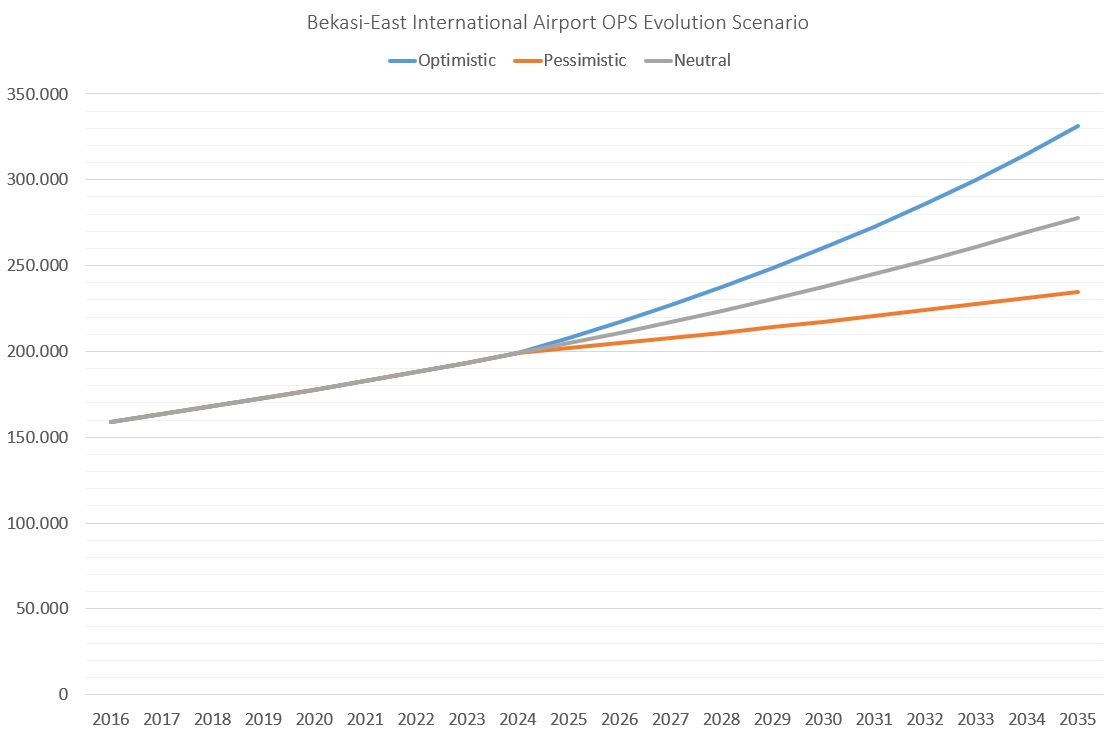
\includegraphics[clip, trim=0cm 0cm 0cm 0cm, width=1\textwidth]{./images/PROGNOSIS/TrafficForecast/BE_OPS_Prev_NEUOPTPES}
	\caption{Bekasi-East Jakarta Airport operations prevision for neutral, optimistic and pessimistic scenario.}
	\label{BE_OPS_Prev_NEUOPTPES}
\end{figure}
	
	\subsection{Flights on busy day}
The total number of passenger and operations calculated for the horizon scenario in 2035 are:

\begin{table}[ht!]
	\label{table:'Traffic2035'}
	\centering
\begin{tabular}{|c|c|}
	\hline 
	\multicolumn{2}{|c|}{\textbf{Traffic in 2035}}\tabularnewline
	\hline  
	Passenger & 35.170.379 \tabularnewline
	\hline 
	Operations & 278.011 \tabularnewline
	\hline 
\end{tabular}
	\caption{Traffic of Bekasi-East Jakarta Airport in 2035.}
\end{table}

IATA defines the busy day as the second busiest day in an average week during the peak month. An average weekly pattern of passenger traffic is calculated for that month. Peaks associated with special events such as religious festivals, trade fairs and conventions, and sport events, are excluded.

Having 2015 busy month values of passenger and operations for CGK airport and the total year values, the percentage of peak above mean can be calculated. Supposing this percentage above mean is conserved along time, it is easy to extrapolate the number of passenger and operations in busy day for the new Bekasi-East Airport. The following results are obtained:

\begin{table}[ht!]
	\label{table:'BusyDayPAX'}
	\centering
	\begin{tabular}{|c|c|c|c|}
		\hline 
		\multicolumn{4}{|c|}{\textbf{Bekasi-East Jakarta Airport PAX in 2035}}\tabularnewline
		\hline 
		\textbf{Type} & Domestic & International & Total\tabularnewline
		\hline 
		\textbf{Total Year} & 2.233.960  & 1.253.000  & 3.486.960 \tabularnewline
		\hline 
		\textbf{Mean Month} & 22.568.860  & 12.601.519  & 35.170.379 \tabularnewline
		\hline 
		\textbf{Mean Day} & 1.880.738  & 1.050.127  & 2.930.865 \tabularnewline
		\hline 
		\textbf{Busy Day} & 73.778  & 41.009  & 114.787 \tabularnewline
		\hline 
	\end{tabular}
	\caption{Determination of number of passengers in busy day.}
\end{table}

\begin{table}[ht!]
	\label{table:'BusyDayOPS'}
	\centering
	\begin{tabular}{|c|c|c|c|}
		\hline 
		\multicolumn{4}{|c|}{\textbf{Bekasi-East Jakarta Airport OPS in 2035}}\tabularnewline
		\hline 
		\textbf{Type} & Domestic & International & Total\tabularnewline
		\hline 
		\textbf{Total Year} & 176.525  & 101.486  & 278.011 \tabularnewline
		\hline 
		\textbf{Mean Month} & 14.710  & 8.457  & 23.168 \tabularnewline
		\hline 
		\textbf{Mean Day} & 484  & 278  & 762 \tabularnewline
		\hline 
		\textbf{Mean Hour} & 24  & 14  & 38 \tabularnewline
		\hline 
		\textbf{Max Hour} & 30  & 20  & 50 \tabularnewline
		\hline 
	\end{tabular}
	\caption{Determination of maximum number of operations per hour.}
\end{table}

With the number of maximum hourly operations and an utilisation factor of 77\% for both domestic and international flights, the number of maximum passenger per hour in the airport is calculated.

\begin{table}[ht!]
	\label{table:'PAXperhour'}
	\centering
\begin{tabular}{|c|c|c|c|}
	\hline 
	\multicolumn{4}{|c|}{\textbf{Bekasi-East Jakarta Airport Peak Hour}}\tabularnewline
	\hline 
	\textbf{Type} & Domestic & International & All\tabularnewline
	\hline 
	\textbf{Utilisation Factor} & 77\% & 77\% & -\tabularnewline
	\hline 
	\textbf{Max PAX/OPS} & 189 & 189 & -\tabularnewline
	\hline 
	\textbf{PAX/OPS} & 146 & 146 & -\tabularnewline
	\hline 
	\textbf{Max PAX/H} & 4.394 & 2.870 & 7.264\tabularnewline
	\hline 
\end{tabular}
\caption{Determination of the peak hour passenger value.}
\end{table}

	
	